%%%%%%%%%%%%%%%%%%%%%%%%%%%%%%%%%%%%%%%%%%%%%%%%%%%%%%%%%%%%%%%%%%%%%%%%
%%
%% main.tex
%% LaTeX-2e 専用
%% 
%% 
%%        設計工学研究室 学位論文テンプレート
%%
%%                      作成日時    2018年 10月 1日
%%
%%%%%%%%%%%%%%%%%%%%%%%%%%%%%%%%%%%%%%%%%%%%%%%%%%%%%%%%%%%%%%%%%%%%%%%%

\documentclass[12pt, a4paper, titlepage]{jsbook}      %ドキュメントクラス

%パッケージ
\usepackage[dvips]{graphicx, color}
\usepackage{amsmath}
\usepackage{amssymb}
\usepackage{array}
\usepackage{hhline}
\usepackage{afterpage}
\usepackage{enumerate}
\usepackage{multicol}
\usepackage{fancyhdr}
\usepackage{subfigure}
\usepackage{bm} %ベクトル表示
\usepackage{slashbox}

%新定義コマンド
\newcommand{\sankou}[1]{$ ^{\text{[#1]}} $}
\newcommand{\chref}[1]{第~\ref{#1}~章}
\newcommand{\secref}[1]{\ref{#1} (p.\pageref{#1})}
\newcommand{\tableref}[1]{(Table.\ref{#1})}
\newcommand{\figref}[1]{(Fig.\ref{#1})}
\newcommand{\figpref}[1]{(Fig.\ref{#1} p.\pageref{#1})}
\newcommand{\degree}{\char'27\kern-.3em\hbox{C}} 

%再定義コマンド
\renewcommand{\figurename}{Fig.~}
\renewcommand{\tablename}{Table.~}
\renewcommand{\labelitemi}{・}
\renewcommand{\labelenumi}{(\theenumi)}

\renewcommand{\eqref}[1]{式 (\ref{#1})}

\renewcommand{\subfigtopskip}{0mm}%図と図の間
\renewcommand{\subfigcapskip}{0mm}%図と副題の間

%余白変更
\setlength{\textwidth}{\fullwidth}
\setlength{\evensidemargin}{\oddsidemargin}

\title{学位論文のテンプレート}
\author{埼玉大学 工学部 機械工学科
        \\
        埼玉 太郎
        }

\begin{document}

    %タイトル
    %%%%%%%%%%%%%%%%%%%%%%%%%%%%%%%%%%%%%%%%%%%%%%%%%%%%%%%%%%%%%%%%%%%%%%%%
%%
%% 題目.tex
%% LaTeX-2e 専用
%% 
%% 
%%        設計工学研究室 学位論文テンプレート
%%
%%                      作成日時    2020年 2月 11日
%%
%%%%%%%%%%%%%%%%%%%%%%%%%%%%%%%%%%%%%%%%%%%%%%%%%%%%%%%%%%%%%%%%%%%%%%%%
\thispagestyle{empty}
\newcommand{\ctext}[1]{\textcolor[rgb]{0.65, 0.65, 0.65}{\raise0.2ex\hbox{\textcircled{\scriptsize{#1}}}}}
%% 卒業論文題目     
\begin{center}
        {\huge 埼玉大学 工学部} \\
        {\huge 機械工学科} \\        
        \vspace{10mm}
        {\Huge 令和5年度 \quad 卒業論文}\\
        \vspace{10mm} 
        
        {\Huge ○○○○○○○○○○の研究} \\
        \vspace{10mm}
        {\LARGE Study on XXXXXXXXXX} \\        
        \vspace{35mm} %題目の長さに応じて適宜修正すること
 \end{center}
        
 \begin{table}[!h]
        \begin{flushright}        
        \renewcommand{\arraystretch}{1.5}
        \begin{tabular}{|c|cc|}
            \hline
            {\Large 学科長}    & {\Large  荒居善雄 教授 \quad} & {\Large\ctext{印}}\\        
            \hline
            {\Large 主指導教員} & {\Large  琴坂信哉 准教授 } &{\Large\ctext{印}}\\
            \hline
            {\Large 副指導教員} & {\Large  程島竜一 准教授 }& \\
            \hline
        \end{tabular}
        \renewcommand{\arraystretch}{1.0}        
    \end{flushright}        
 \end{table}
\begin{table}[!b]
        \begin{flushright}
        \renewcommand{\arraystretch}{1.2}
        \begin{tabular}{|c|c|}
            \hline
             {\Large 提出日} & {\Large 2023年2月XX日}\\ %年は西暦で記載
             \hline
             {\Large 研究室} & {\Large 設計工学 }\\
             \hline
             {\Large 学籍番号} & {\Large 20TM028}\\
             \hline
             {\Large 氏  名} & {\Large 長谷川 大晴}\\
            \hline
        \end{tabular}
        \renewcommand{\arraystretch}{1.0}
        \end{flushright}
\end{table}
                                %タイトル ※修士は題目_修士、学士は題目_学士に変更すること。編集するファイルもそれぞれ対応するファイルを編集する。

    \frontmatter
    \tableofcontents
    \listoffigures
    \listoftables
    \mainmatter{} 
    %!!重要!!
    %各章は奇数ページから開始するように調整すること
    %つまり各章は偶数ページで終わるように、改ページ等を使用して調整する。
    %%%%%%%%%%%%%%%%%%%%%%%%%%%%%%%%%%%%%%%%%%%%%%%%%%%%%%%%%%%%%%%%%%%%%%%%
%%
%% 序論.tex
%% LaTeX-2e 専用
%% 
%% 
%%        設計工学研究室 学位論文テンプレート
%%
%%                      作成日時    2010年 12月 17日
%%
%%%%%%%%%%%%%%%%%%%%%%%%%%%%%%%%%%%%%%%%%%%%%%%%%%%%%%%%%%%%%%%%%%%%%%%%

\chapter{序論}\label{chapter:序論}
第\ref{chapter:序論}章では,本研究の研究背景と先行研究,そして研究の目的を述べる.


\section{背景}
近年,人間に代わって作業を行う移動ロボットの導入が進められている.
これらのロボットの多くはタイヤやホイールを用いての移動を行うが,その他の移動様式として,脚を使用して移動を行う多脚ロボットが存在する.
多脚ロボットは他の移動様式を用いて移動するロボットに比べて,障害物をまたいで超えることが可能な点や,離散的に接地点を選択できる点において優れているといえる.

実際に,林業を行う山間地において多脚ロボットの導入を

このような不整地において,多脚ロボットを使用する場合は適切な歩容計画を行う必要がある.
歩容計画には,カムやリンクを用いて,周期的に脚を動かす固定歩容と,
非周期的に脚を動かす自由歩容がある.

当研究室で行われてきた先行研究では,

\section{本研究の目的}
これまでの研究によって,3次元の不整地において,重心高さを変更しつつ,
自由歩容パターン生成を行うことが可能となった.
しかし低頻度ではあるが,グラフ探索に成功したとしても,
その歩容パターン通りに歩行することができずに動作を停止してしまう問題が生じてしまった.

そこで本論文では,常に脚軌道生成に成功するような歩容パターン生成手法を提案し,
脚軌道生成の失敗による動作停止を防ぐことを目的とする.

\section{本論文の構成}
本論文は,全6章から構成される.

第2章「歩容パターンの再評価手法の提案」では,~を述べる.
第3章「実験装置や開発機械」では,~を述べる.
第4章「実験」では,~を述べる.
第5章「結論」では本論文の結論と今後の課題を述べる.

% \section{other}
% 図の参照はFig. \ref{fig:sample}とする.

% 表の参照はTab. \ref{table:sample}とする.

% 参考文献の参照は\cite{実用的4足歩行機械}とする.



% %図の挿入例
% \begin{figure}[tbp]
%   \begin{center}
%     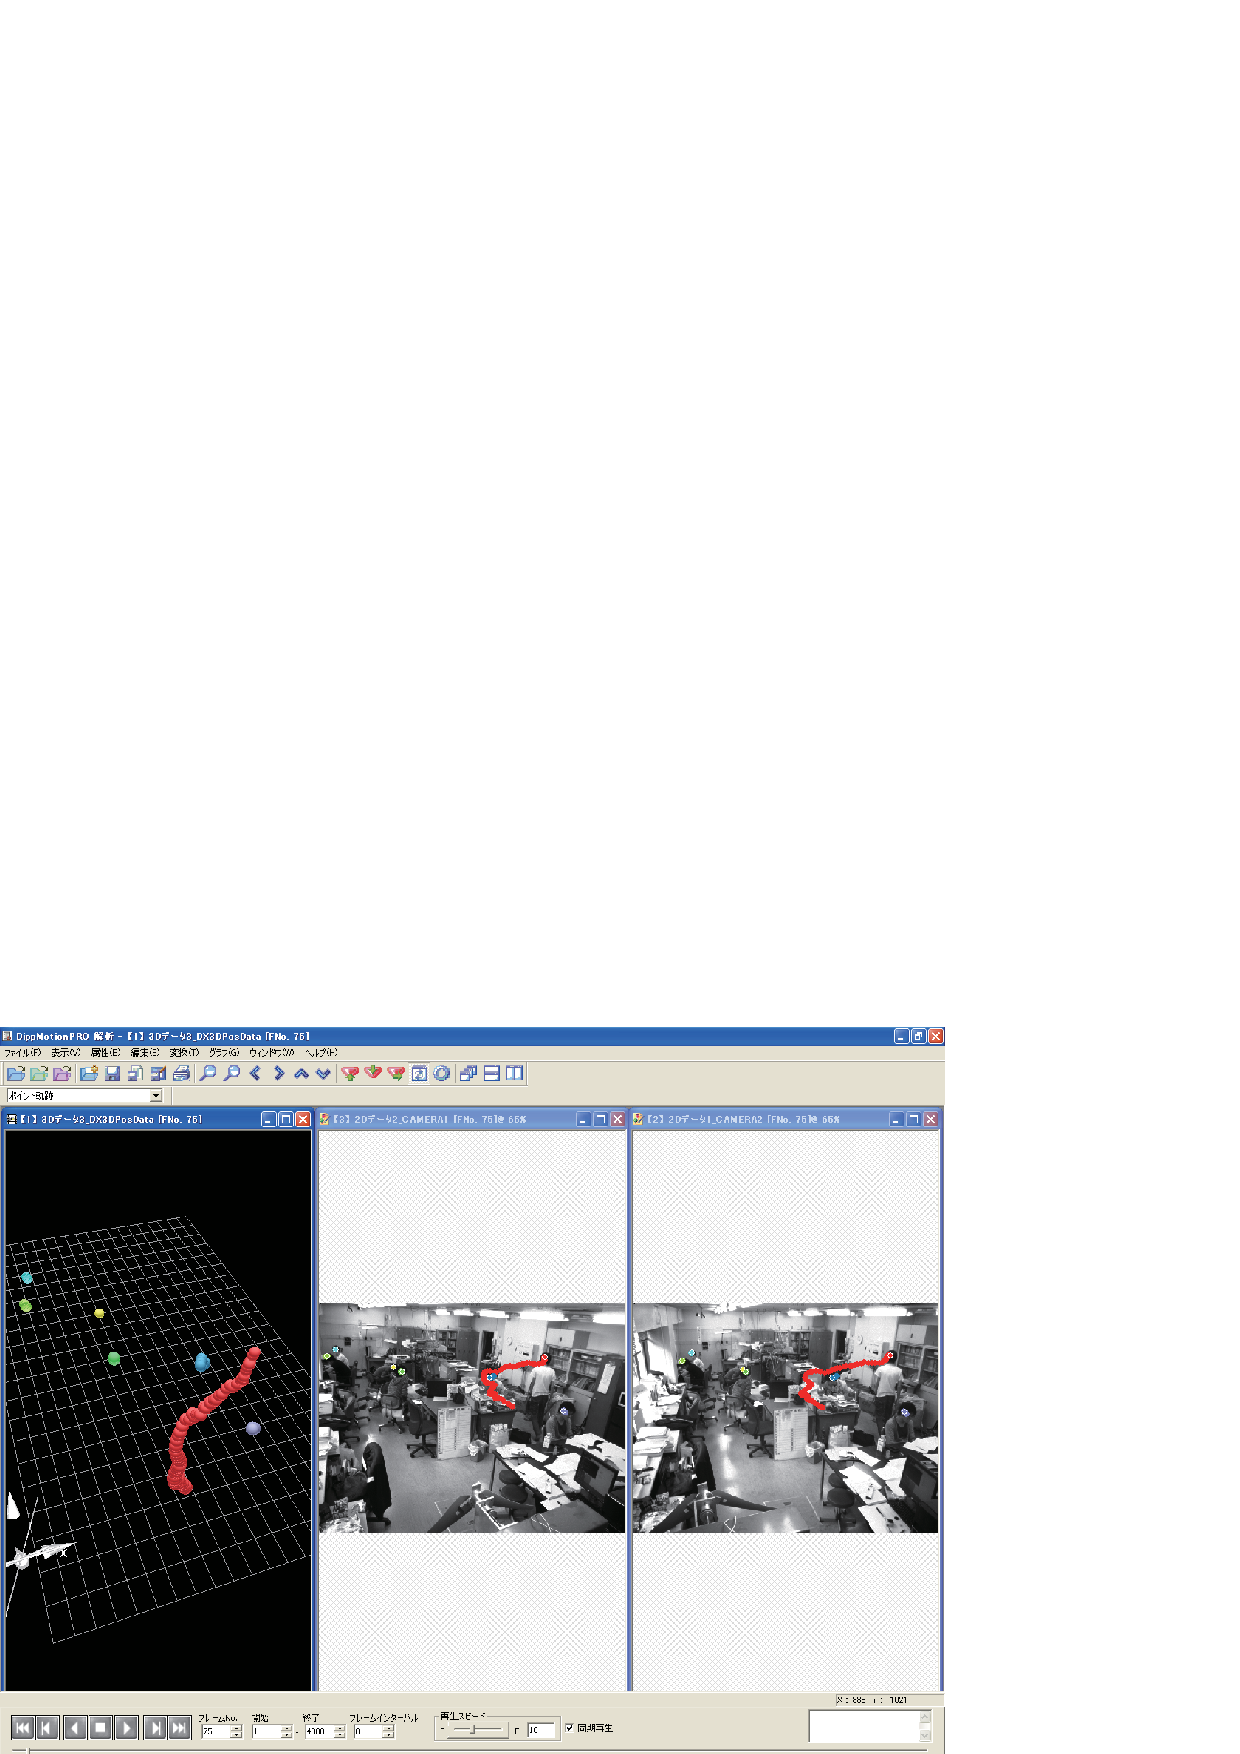
\includegraphics[width=50mm, clip]{figure1/sample.jpg}
%     \caption{Sample figure}
%     \label{fig:sample}
%   \end{center}
% \end{figure}

% %表の挿入例
% \begin{table}[tbp]
%     \caption{Sample table}
%     \label{table:sample}
%     \begin{center}
%         \begin{tabular} {|c|c|c|}
%         \hline
%         Item & Spec. & Quantity  \\
%         \hline\hline
%         A & high & 10 \\
%         \hline
%         B & low & 100 \\
%         \hline
%         \end{tabular}
%     \end{center}
% \end{table}
                                          %第1章
    %% 歩容パターンの再評価手法の提案.tex
%% LaTeX-2e 専用

%% 全体の流れとしては,まず,先行研究の問題点を指摘し,次に,歩容パターンの再評価手法を提案する.

\chapter{歩容パターンの再評価手法の提案}\label{chapter:歩容パターンの再評価手法の提案}
第\ref{chapter:歩容パターンの再評価手法の提案}章では,先行研究の手法およびその問題点を指摘し,
常に脚軌道生成が可能な自由歩容パターン生成手法として,歩容パターンの再評価手法を述べる.

% 先行研究の章
\section{本研究室における自由歩容パターン生成の先行研究}
\subsection{グラフ理論について}
グラフとは,頂点(ノード)とそれらを結ぶ辺(エッジ)からなる図形である.
このグラフを用いて,さまざまな問題を取り扱う学問をグラフ理論という.

以降の説明を簡単にするため,この論文で用いるグラフ理論の用語について簡潔に述べる.
エッジに向きがあるものを有向グラフ,逆に向きを持たないものを無向グラフという.
また,閉路を持たず,かつ,すべての頂点間に経路が存在するグラフを木という.
このような木構造をもつグラフのうち,図\ref*{fig:tree_graph}のように,
根となるノードを持ち,そのノードからすべてのノードに到達可能なものを根付き木という.

根付き木において,あるノードから遷移可能なノードをそのノードの子ノードと呼ぶ.
逆に,あるノードに遷移可能なノードをそのノードの親ノードと呼ぶ.
親ノードを持たないノードを根ノードと呼び,子ノードを持たないノードを葉ノードと呼ぶ.
また,あるノードから根ノードまでのエッジの数をそのノードの深さと呼び,
根ノード自身の深さは0となる.

図\ref*{fig:tree_graph}においては,ノードAが根ノードであり,ノードB,Cがその子ノードである.
また,ノードB,ノードD,E,ノードCはノードFを子ノードとして持ち,ノードD,E,Fは葉ノードである.
ノードAの深さは0であり,ノードB,Cの深さは1,ノードD,E,Fの深さは2となる.

グラフのあるノードから別のノードに到達するための経路をパスと呼び,
これを求めることをグラフ探索と呼ぶ.
グラフ探索には,深さ優先探索,幅優先探索などのさまざまなアルゴリズムが存在する.
深さ優先探索では,始点となるノードから,深さが深くなる方向を優先して探索を行う.
これに対して,幅優先探索では,始点となるノードから,深さが浅いノードを優先して探索を行う手法である.

\begin{figure}[tbp]
  \begin{center}
    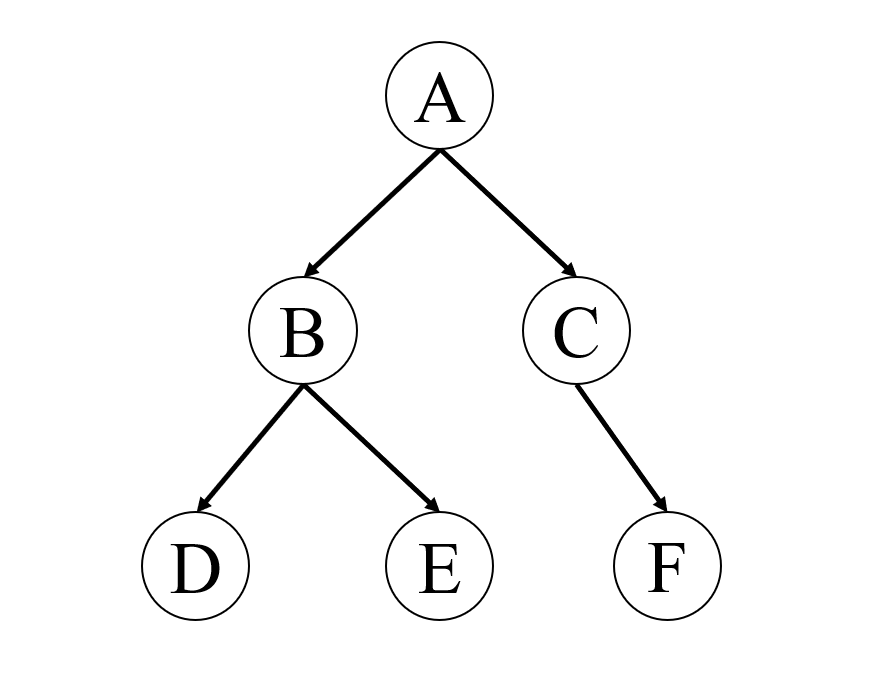
\includegraphics[width=50mm, clip]{figure/tree_graph.png}
   \caption{Tree Graph}
    \label{fig:tree_graph}
  \end{center}
\end{figure}

\subsection{歩容パターングラフの定義}
本研究においては,6脚ロボットの歩容パターンをグラフを用いて表現する.
ロボットの状態をノードとし,ロボットの状態間の遷移,つまりロボットの動作をエッジとして表現する.
また,グラフは有向の根付き木とする.このようにして作られたグラフを歩容パターングラフと定義する.

グラフ探索がよく用いられる題材は路線図や回路図などであり,ノードの数が有限であるものである.
しかし,歩容パターングラフはロボットの状態や動作を対象とするため,
無限の組み合わせが存在する.
そのため,先行研究では状態や動作を離散化することで歩容パターン生成をグラフへ落とし込んでいる.
以下に各要素の離散化について述べる.

\subsubsection{脚位置の離散化}

\subsubsection{グラフの階層構造}
\subsubsection{エッジの離散化}
\subsubsection{脚軌道生成の分離}

\subsection{脚軌道生成の失敗}


% 予備実験の章
\section{歩行シミュレーションによる脚軌道生成失敗時の脚先位置の特定}

\subsection{シミュレーション実験の目的}
脚軌道生成の失敗を防ぐためには,脚軌道生成の失敗時の脚先の座標を特定する必要がある.
そのため,予備実験として先行研究と同じ条件で歩行シミュレーション実験を行い,失敗の原因を考察した.

\subsection{シミュレーションの条件}

\subsection{シミュレーションの結果}
以下の図に脚軌道生成失敗時の脚先の座標を示す.

\subsection{脚軌道生成の失敗の原因の考察}

\section{常に脚軌道生成が可能な自由歩容パターン生成手法の検討}
常に脚軌道生成を可能にするためには,近似された脚可動範囲を適切に設定する必要がある.


\section{歩容パターンの再評価手法}

                     %第2章
    %%%%%%%%%%%%%%%%%%%%%%%%%%%%%%%%%%%%%%%%%%%%%%%%%%%%%%%%%%%%%%%%%%%%%%%%
%%
%% 実験装置や開発機械.tex
%% LaTeX-2e 専用
%% 
%% 
%%        設計工学研究室 学位論文テンプレート
%%
%%                      作成日時    2010年 12月 17日
%%
%%%%%%%%%%%%%%%%%%%%%%%%%%%%%%%%%%%%%%%%%%%%%%%%%%%%%%%%%%%%%%%%%%%%%%%%

\chapter{実験装置や開発機械}\label{chapter:実験装置や開発機械}
第\ref{chapter:実験装置や開発機械}章では,~を述べる.

\section{全体機能とサブ機能の構造}
\section{○○機能の設計}
\section{××機能の開発}
\section{△△機能の実現}



            %第3章
    %%%%%%%%%%%%%%%%%%%%%%%%%%%%%%%%%%%%%%%%%%%%%%%%%%%%%%%%%%%%%%%%%%%%%%%%
%%
%% 実験.tex
%% LaTeX-2e 専用
%% 
%% 
%%        設計工学研究室 学位論文テンプレート
%%
%%                      作成日時    2010年 12月 17日
%%
%%%%%%%%%%%%%%%%%%%%%%%%%%%%%%%%%%%%%%%%%%%%%%%%%%%%%%%%%%%%%%%%%%%%%%%%

\chapter{実験}\label{chapter:実験}
第\ref{chapter:実験}章では,~を述べる.

\section{○○の実験}
\subsection{○○の実験目的}
\subsection{○○の実験手順}
\subsection{○○の実験結果}
\subsection{○○の実験考察}

\section{××の実験}
                                          %第4章
    %%%%%%%%%%%%%%%%%%%%%%%%%%%%%%%%%%%%%%%%%%%%%%%%%%%%%%%%%%%%%%%%%%%%%%%%
%%
%% 結論.tex
%% LaTeX-2e 専用
%% 
%% 
%%        設計工学研究室 学位論文テンプレート
%%
%%                      作成日時    2010年 12月 17日
%%
%%%%%%%%%%%%%%%%%%%%%%%%%%%%%%%%%%%%%%%%%%%%%%%%%%%%%%%%%%%%%%%%%%%%%%%%

\chapter{結論}\label{chapter:結論}

\section{結論}

本論文では,~~を論じた.

第1章「序論」では,~を述べた.
第2章「理論と実施計画」では,~を述べた.
第3章「実験装置や開発機械」では,~を述べた.
第4章「実験」では,~を述べた.
第5章「結論」では本論文の結論と今後の課題を述べた.

\section{今後の課題}
                                          %第5章
    %%%%%%%%%%%%%%%%%%%%%%%%%%%%%%%%%%%%%%%%%%%%%%%%%%%%%%%%%%%%%%%%%%%%%%%%
%%
%% 付録.tex
%% LaTeX-2e 専用
%% 
%% 
%%        設計工学研究室 学位論文テンプレート
%%
%%                      作成日時    2010年 12月 17日
%%
%%%%%%%%%%%%%%%%%%%%%%%%%%%%%%%%%%%%%%%%%%%%%%%%%%%%%%%%%%%%%%%%%%%%%%%%

\appendix
%%%%%%%%%%%%%%%%%%%%%%%%%%%%%%%%%%%%%%%%%%%%%%%%%%%%%%%%%%%%%%%%%%%%%%%%
%%
%% 付録.tex
%% LaTeX-2e 専用
%% 
%% 
%%        設計工学研究室 学位論文テンプレート
%%
%%                      作成日時    2010年 12月 17日
%%
%%%%%%%%%%%%%%%%%%%%%%%%%%%%%%%%%%%%%%%%%%%%%%%%%%%%%%%%%%%%%%%%%%%%%%%%

\chapter{C++20への移行}\label{chapter:付録A}
\section{C++20の新機能}
C++にはコンパイラの標準規格として,C++98,C++03,C++11などが存在する.
その中でもC++11以降は約3年に一度のペースで新しい規格が策定されている.
先行研究のプログラムでは,C++17を使用していたが,本研究ではC++20\cite{Thomas_C++20}を使用するように変更を行った.
C++20では,C++17からの変更点として,以下のようなものがある.
\begin{itemize}
  \item constexpr関数の制限緩和
  \item 標準ライブラリの多くの関数がconstexpr関数に変更
  \item conceptの導入
  \item std::number,std::formatの導入
\end{itemize}
これらの機能を使用することで,プログラムの最適化を行うことができる上,可読性を向上されることができる.
以下に各機能の詳細を記述する.

\section{constexpr変数・関数}
constexpr関数はコンパイル時に評価される関数であり,
C言語におけるマクロ関数のような処理を実現するために使用される.
たとえば,以下のようなプログラムを考える.

\newpage  % 改ページする

\begin{lstlisting}[caption=convert func as macro,label=convert_func_as_macro]
#include <iostream>

// defined as macro
#define CONVERT_TO_RAD(deg) (deg * 3.1415926535f / 180.0f)  

int main()
{
  float deg = 90.0f;
  
  // It will deploy deg * 3.1415926535f / 180.0f.
  std::cout << CONVERT_TO_RAD(deg) << std::endl;
}
\end{lstlisting}

% 1行開ける
\vskip \baselineskip

このプログラムでは,マクロ関数を使用して,度数法で表された角度をラジアンに変換している.
プログラムを記述する際にはラジアンで角度を表現すると可読性が低くなるため,
度数法で記述することによる利点は大きいが,実際の処理ではラジアンで角度を表現する必要があるので,
このようなマクロが実際に使用されることは多いだろう.

しかし,マクロにはいくつかの問題点がある.
まず1つとして,マクロは常にグローバルスコープで定義されることである.
通常C++の開発においては,クラスや名前空間を使用して,変数や関数をスコープを限定して定義することが多い.
スコープを限定することは,変数や関数の名前が衝突することを防ぐことができるため,
大規模な開発や複数のライブラリを使用する場合には必須である.
だが,マクロは名前空間内に定義したとしてもグローバルスコープに展開されるため,
名前の衝突を防ぐことができないのである.

もう1つの問題点は,マクロは型の確認を行わないことである.
C++はpythonやjava scriptなどの動的型付け言語とは異なり静的型付け言語である.
そのため,コンパイル時に型の不一致や意図しないキャストを警告として出力することができ,
ランタイムエラーを防ぐことができる.
しかし,マクロはプリコンパイル時に文字を置換するだけであるため,型の確認を行わない.
そのためたとえば上記のマクロ関数において,引数をint型やdouble型,果てはその他のクラスなどに変更しても,
float型との掛け算演算子が定義されていればコンパイルは通ってしまう.
先行研究のプログラムではマクロ関数を使用している箇所が多く存在したため,
実際に浮動小数点型のfloat型とdouble型が混在している箇所が存在した.

これをconstexpr関数を使用することで,以下のように書き換えることができる.

\newpage  % 改ページする

\begin{lstlisting}[caption=convert func as constexpr,label=convert_func_as_constexpr]
#include <iostream>

// defined as constexpr function
constexpr float ConvertToRad(float deg)
{
  return deg * 3.1415926535f / 180.0f;
}

int main()
{
  // declared as constexpr variable
  constexpr float deg = 90.0f;
  
  // It will deploy 1.57079632675f.
  std::cout << ConvertToRad(deg) << std::endl;
}
\end{lstlisting}

% 1行開ける
\vskip \baselineskip

このようにconstexpr関数を使用することで,マクロ関数のようにコンパイル時に評価される関数を定義することができる.
また,constexpr関数はコンパイル時に評価が行われるため,コンパイル時に型の確認を行うことができる.
加えて,constexpr関数はスコープを限定することができるため,名前の衝突を防ぐことができる.

以上のようにマクロの持つ問題点を解決することができるが,constexpr関数の本当の利点はコンパイル時に処理が実行されることである.
\ref{convert_func_as_constexpr}の14,15行目にあるように,引数を含めてコンパイル時に評価が可能であれば,
コンパイル時に関数が実行される.そのため,関数の呼び出しによるオーバーヘッドを削減することができる.



\chapter{PhantomX Mark I\hspace{-1.2pt}Iのサーボモータ}\label{chapter:B}
\section{サーボモータの仕様}

PhantomX Mark I\hspace{-1.2pt}Iは計18個のサーボモータを搭載しており,
Dynamixel AX-12A,あるいはDynamixel AX-18Aを搭載したモデルがある.
今回使用したのはDynamixel AX-18Aを搭載したモデルであるため,
以下にDynamixel AX-18Aの仕様をまとめたWebページを掲載する.
(https://e-shop.robotis.co.jp/product.php?id=235 アクセス日 2023/9/15)

\begin{figure}
  \centering
  \begin{tabular}{cc}
    \fbox{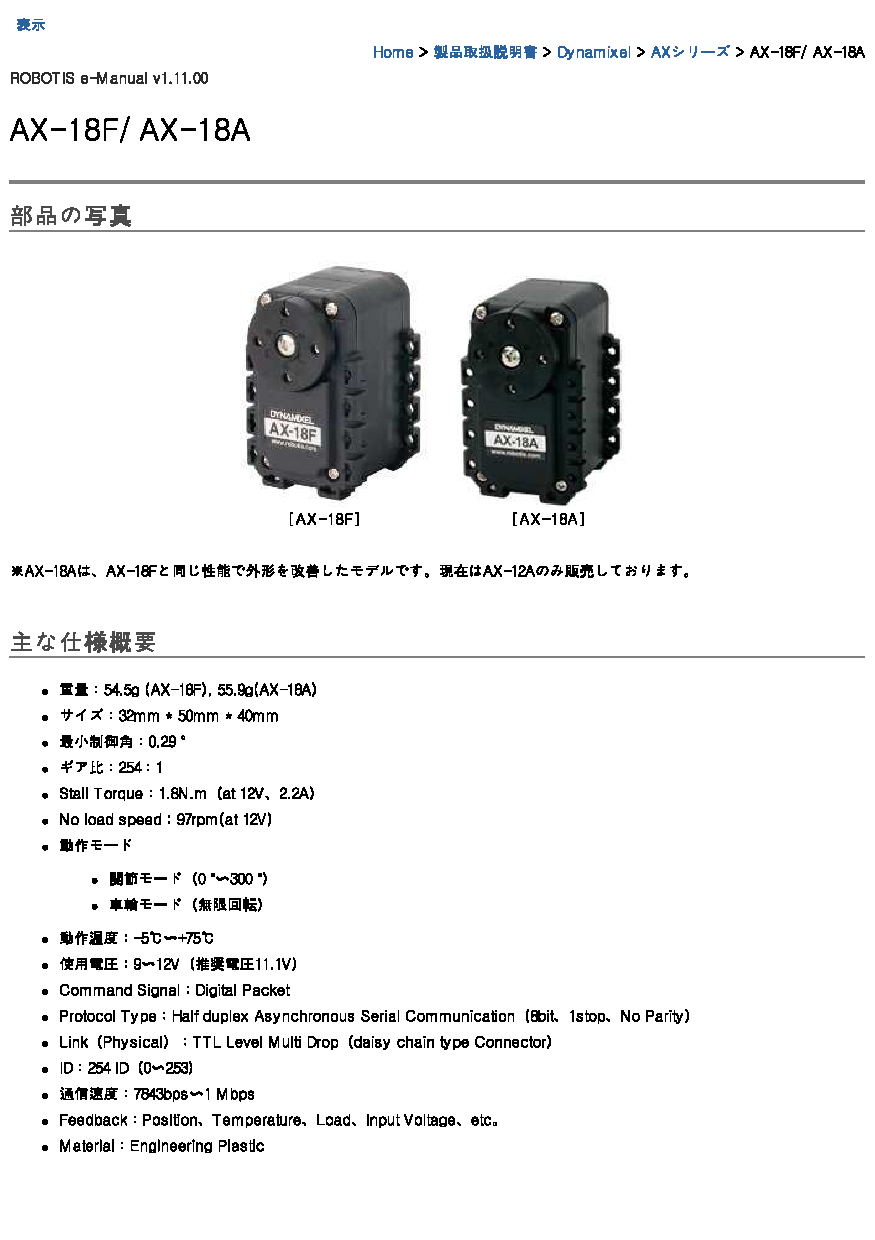
\includegraphics[page=1, width=0.4\textwidth]{web_page/AX-18A_Manual.pdf}} &
    \fbox{\includegraphics[page=2, width=0.4\textwidth]{web_page/AX-18A_Manual.pdf}} \\
    Page 1 & Page 2 \\
  \end{tabular}

  \caption{Dscription AX-18A (page1--2)}
  \label{fig:ax-18_1-2}  % chktex 24
\end{figure}

\begin{figure}
  \centering
  \begin{tabular}{cc}
    \fbox{\includegraphics[page=3, width=0.4\textwidth]{web_page/AX-18A_Manual.pdf}} &
    \fbox{\includegraphics[page=4, width=0.4\textwidth]{web_page/AX-18A_Manual.pdf}} \\
    Page 3 & Page 4 \\
    \fbox{\includegraphics[page=5, width=0.4\textwidth]{web_page/AX-18A_Manual.pdf}} &
    \fbox{\includegraphics[page=6, width=0.4\textwidth]{web_page/AX-18A_Manual.pdf}} \\
    Page 5 & Page 6 \\
  \end{tabular}

  \caption{Dscription AX-18A (page3--6)}
  \label{fig:ax-18_3-6}  % chktex 24
\end{figure}

\begin{figure}
  \centering
  \begin{tabular}{cc}
    \fbox{\includegraphics[page=7, width=0.4\textwidth]{web_page/AX-18A_Manual.pdf}} &
    \fbox{\includegraphics[page=8, width=0.4\textwidth]{web_page/AX-18A_Manual.pdf}} \\
    Page 7 & Page 8 \\
    \fbox{\includegraphics[page=9, width=0.4\textwidth]{web_page/AX-18A_Manual.pdf}} &
    \fbox{\includegraphics[page=10, width=0.4\textwidth]{web_page/AX-18A_Manual.pdf}} \\
    Page 9 & Page 10 \\
  \end{tabular}

  \caption{Dscription AX-18A (page7--10)}
  \label{fig:ax-18_7-10}  % chktex 24
\end{figure}

\begin{figure}
  \centering
  \begin{tabular}{cc}
    \fbox{\includegraphics[page=11, width=0.4\textwidth]{web_page/AX-18A_Manual.pdf}} &
    \fbox{\includegraphics[page=12, width=0.4\textwidth]{web_page/AX-18A_Manual.pdf}} \\
    Page 11 & Page 12 \\
    \fbox{\includegraphics[page=13, width=0.4\textwidth]{web_page/AX-18A_Manual.pdf}} & 
    \\
    Page 13 &  \\
  \end{tabular}

  \caption{Dscription AX-18A (page11--13)}
  \label{fig:ax-18_11-13}  % chktex 24
\end{figure}

% 改ページする
\clearpage
 

% \section{計算手順}

% \chapter{脚機構図面}\label{chapter:付録B}
% \section{組図}
% \section{断面図}
                                          %付録(あれば)
    \backmatter{}                                                %章番号を付けない
    
\chapter*{謝辞}\label{chapter:謝辞}
\addcontentsline{toc}{chapter}{謝辞}

本論文の研究と執筆にあたりその細部に至るまで終始懇切なる御指導と御鞭撻を賜りました,
埼玉大学大学院理工学研究科琴坂信哉准教授,程島竜一准教授に謹んで深謝の意を申し上げます.

また,研究室において常に熱心な御討論を頂きました,OB・学生の方々に感謝の意を表します.
                                          %謝辞
    \begin{thebibliography}{99}
    \bibitem{Sotnik_Prospects_for_Introduction}
    Sotnik S, Lyashenko V:
    ``Prospects for Introduction of Robotics in Service'',
    International Journal of Academic Engineering Research.
    Vol.6,
    pp.4-9, % chktex 8
    2022.

    \bibitem{Pudu_BellaBot}
    Pudu Robotics Inc:
    ``BellaBot'',
    https://www.pudurobotics.com/jp/products/bellabot (参照2024/01/23).

    \bibitem{Locomotion_for_difficult_terrain}
    Freyr Hardarson:
    ``Locomotion for difficult terrain'',
    1997.

    \bibitem{Boston_Dynamics_Spot}
    Boston Dynamics Inc:
    ``Spot®'',
    https://bostondynamics.com/products/spot/ (参照2024/01/23).

    \bibitem{NEDO}
    国立研究開発法人 新エネルギー・産業技術総合開発機構:
    ``NEDO 先導研究プログラム 2021年度'',
    Vol.1,
    p.57, 
    2022. 

    \bibitem{J_Kim_Dexterous_Crabster}
    B. H. Jun, Hyungwon Shim:
    ``A Dexterous Crabster Robot Explores the Seafloor'',
    The ACM Magazine for Students,
    Vol.20,
    pp.38--45,
    2014.

    \bibitem{J_Kim_Little_Crabster}
    J. Y. Kim, B. H. Jun:
    ``Mechanical Design of Six-Legged Walking Robot, Little Crabster'',
    Oceans-Yeosu,
    pp.1--8,
    2012.

    \bibitem{Hirose_Static_stability_criterion}
    広瀬,塚越,米田: 
    ``不整地における歩行機械の静的安定性評価基準'', 
    J. of Robotic Systems,
    Vol.16, No.8, 
    pp.1076--1082,
    1998.

    \bibitem{Prabir_Graph_search}
    Prabir K. Pal, K. Jayarajan: 
    ``Generation of Free Gait A Graph Search Approach'',
    IEEE Transactions on Robotics and Automation,
    Vol.7, No.3,
    1991.

    \bibitem{Prabir_Graph_search_Six}
    Prabir K. Pal, V. Mahadev and K. Jayarajan:
    ``Gait generation for a six-legged walking machine through graph search'',
    Proceedings of the 1994 IEEE International Conference on Robotics and Automation,
    vol.2,
    pp.1332--1337,
    1994.

    \bibitem{Arata_Graph_search_Six}
    新, 田窪, 上野:
    ``障害物環境下におけるトライポッド歩容の脚配置計画'',
    ロボティクス・メカトロニクス講演会講演概要集,
    2015.

    \bibitem{Oki_Graph_search}
    大木,程嶋,琴坂: 
    ``多脚ロボットの不整地踏破を目標とするグラフ探索を用いた歩行パターン生成'', 
    ロボティクス・メカトロニクス講演会講演概要集,
    2015.   

    \bibitem{Nakaoka_Graph_search}
    中岡,程嶋,琴坂: 
    ``不整地における特定位置・脚着地点への遷移を目的とした多脚歩行ロボットの歩行動作計画'',
    日本機械学会関東支部総会講演会講演論文集,
    2016.

    \bibitem{Shina_Graph_search}
    椎名,程嶋,琴坂: 
    ``グラフ探索を用いた多脚ロボットの旋回歩容パターン生成'',
    日本機械学会関東支部総会講演会講演論文集,
    2018.

    \bibitem{Miura_Graph_search}
    三浦,程嶋,琴坂: 
    ``グラフ探索による多脚歩行ロボットの自由歩容パターン生成 第4報:出現頻度によるノード枝刈りを用いた探索時間の短縮'',
    日本機械学会関東支部総会講演会講演論文集,
    2019.

    \bibitem{Hato_Graph_search}
    波東,程嶋,琴坂: 
    ``グラフ探索による多脚歩行ロボットの自由歩容パターン生成 第5報: 重心の上下移動のエッジを用いた重心高さの変更'',
    日本機械学会関東支部総会講演会講演論文集,
    2020.

    \bibitem{Program_Challenge_Book}
    秋葉, 岩田, 北川:
    ``プログラミングコンテストチャレンジブック'',
    毎日コミュニケーションズ,
    2010.
    
    \bibitem{Dxlib_Web}
    DXライブラリ置き場.
    https://dxlib.xsrv.jp/ (参照2024/01/23).

    \bibitem{cita:phantom_x_mark_2}
    Trossen~Robotics:
    ``PhantomX~AX~Hexapod~Mark~II~Kit''.
    \url{https://www.trossenrobotics.com/hex-mk2},
    (参照2024/01/23).

    \bibitem{Thomas_C++20}
    Thomas~Koppe:
    ``Changes~between~C++17~and~C++20~DIS''.
    \url{https://www.open-std.org/jtc1/sc22/wg21/docs/papers/2020/p2131r0.html}, 
    (参照2024/01/23).

    \bibitem{cita:ax_18a_manual}
    ROBOTIS:
    ``AX-18A~User~Manual''.
    \url{https://e-shop.robotis.co.jp/product.php?id=235},
    (参照2023/9/15).

\end{thebibliography}
\endinput                                 %参考文献
\end{document}